\chapter{मूलक, कार्बीन और पुनर्विन्यास}\label{ch:b3:radicals-carbenes}

पाइरेथ्रम डेज़ी क्राइसैन्थेमिक अम्ल के एस्टरों से अपनी रक्षा करती है, जो अणु
एक त्रिसदस्यीय कार्बन वलय के चारों ओर बने होते हैं; उनके संश्लेषित संबंधी
सबसे अधिक प्रयुक्त घरेलू कीटनाशकों में हैं। रसायनज्ञ ऐसे वलयों को एक चरण में
किसी द्विबंध पर \omterm{def:b3:organometallic-bonding:carbene}{कार्बीन} जोड़कर बंद करते हैं: एक ऐसा कार्बन परमाणु जिसके चारों ओर केवल छह इलेक्ट्रॉन
होते हैं, जिनमें से दो असाझा होते हैं। यह अध्याय उन क्रियाशील मध्यवर्तियों का विवेचन करता है
जिनसे प्रथम और द्वितीय वर्ष के खंड केवल प्रसंगवश मिले थे (संश्लेषण में प्रयुक्त
मूलक, \omterm{def:b3:organometallic-bonding:carbene}{कार्बीन} और \omterm{def:b3:radicals-carbenes:nitrene}{नाइट्रीन}), और उन पुनर्विन्यासों का जिनमें कोई समूह किसी
इलेक्ट्रॉन-न्यून कार्बन, नाइट्रोजन या ऑक्सीजन परमाणु पर खिसकता है, जिनमें वे दो भी हैं
जो एक ही कीटोन से नायलॉन-6 और एक जैवनिम्नीकरणीय पॉलिएस्टर के एकलक
बनाते हैं।

\begin{recall}
प्रथम वर्ष के खंड ने मूलक, समांश विखंडन और अर्ध-शीर्ष तीर,
कार्बधनायन और उनके पुनर्विन्यास, नाभिकरागी और निर्गामी समूह प्रस्तुत किए; द्वितीय
वर्ष के खंड ने मूलक शृंखलाएँ (आरंभन, संचरण, समापन, मूलक
आरंभक), पेरॉक्सी अम्ल, लैक्टोन, लैक्टम और इमीन।
\Cref{ch:b3:complex-kinetics} ने शृंखला बलगतिकी का विवेचन किया,
\cref{ch:b3:organometallic-bonding} ने लिगैंड के रूप में \omterm{def:b3:organometallic-bonding:carbene}{कार्बीनों} का,
\cref{ch:b3:many-electron-atoms} ने एकल और \omterm{def:b3:many-electron-atoms:singlet-triplet}{त्रिक अवस्थाओं} का, और
\cref{ch:b3:rate-theories} ने हैमंड अभिगृहीत का।
\end{recall}

\begin{omfigure}
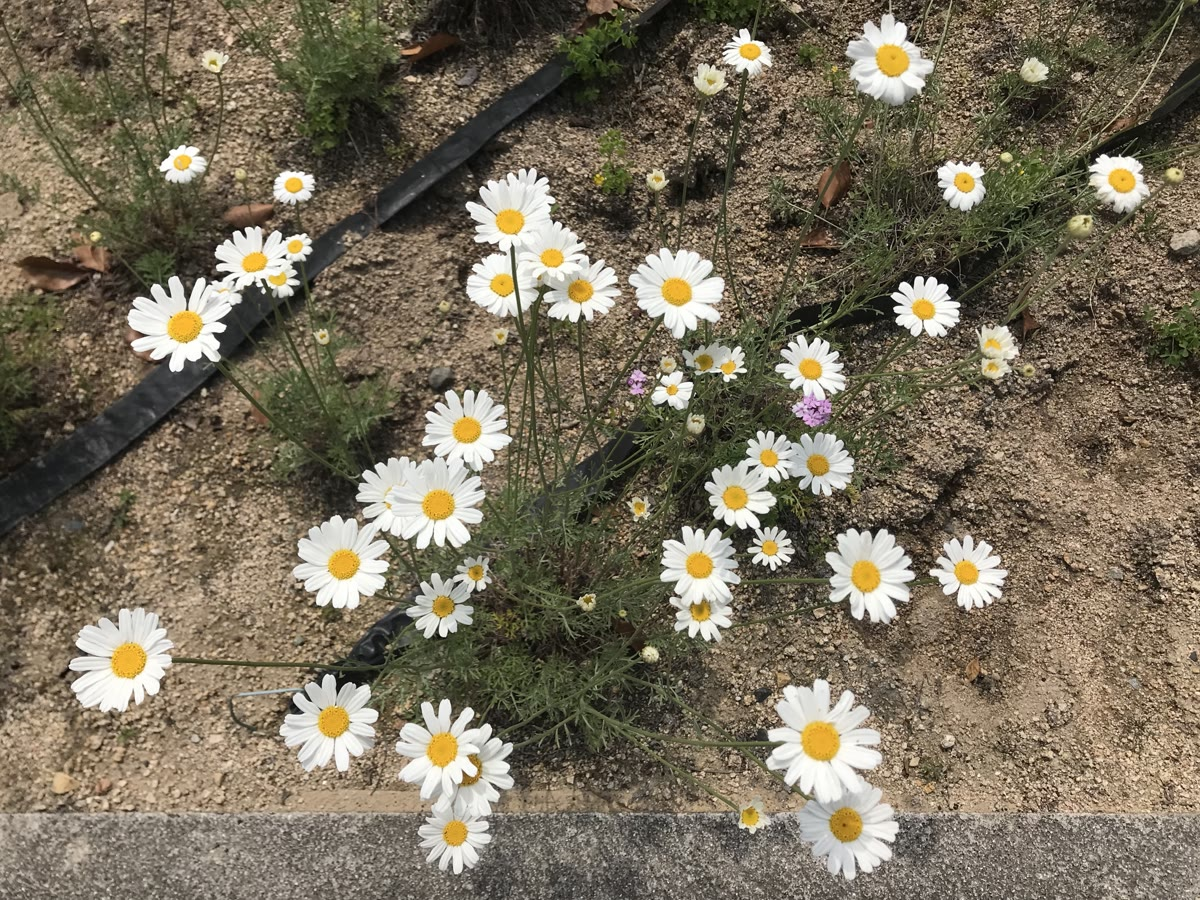
\includegraphics[width=0.48\linewidth]{images/book4/pyrethrum.jpg}

{\small पाइरेथ्रम डेज़ी। इनके फूलों में पाइरेथ्रिन होते हैं, एक साइक्लोप्रोपेनकार्बोक्सिलिक अम्ल के
कीटनाशी एस्टर। छायाचित्र: सोरामिमी, CC BY-SA 4.0।}
\end{omfigure}

\section{संश्लेषण में मूलक शृंखला अभिक्रियाएँ}

किसी कार्बन मूलक का स्थायित्व उस C--H आबंध की आबंध वियोजन
एन्थैल्पी से मापा जाता है जो उसे बनाता: आबंध जितना दुर्बल, मूलक उतना ही
स्थायी।

\begin{proposition}[आबंध वियोजन एन्थैल्पियाँ]\label{prop:b3:radicals-carbenes:bde}
\qty{298}{K} पर R--H की आबंध वियोजन एन्थैल्पी गैस-प्रावस्था संभवन
एन्थैल्पियों से प्राप्त होती है: $\mathrm{BDE(R{-}H)} = \Delta_fH^\circ(\mathrm R^\bullet) + \Delta_fH^\circ(\mathrm H^\bullet) - \Delta_fH^\circ(\mathrm{RH})$।
\end{proposition}

\begin{proof}
समांश विखंडन $\mathrm{RH \to R^\bullet + H^\bullet}$ की अभिक्रिया एन्थैल्पी, हेस के नियम से, उत्पादों के
संभवन की एन्थैल्पी ऋण अभिकारक की संभवन एन्थैल्पी है; परिभाषा से वह अभिक्रिया एन्थैल्पी
आबंध वियोजन एन्थैल्पी है।
\end{proof}

\begin{omfigure}
% ledger: dfh4:CH3r, dfh4:C2H5r, dfh4:iC3H7r, dfh4:tC4H9r, dfh4:PhCH2r, dfh4:H, dfh:CH4_g, dfh:C2H6_g, dfh:C3H8_g, dfh4:iC4H10, dfh4:toluene_g
\begin{tikzpicture}
\begin{axis}[width=0.72\linewidth, height=5.2cm, ybar, bar width=16pt, ymin=350, ymax=450,
  xtick={1,2,3,4,5}, xticklabels={{$\ce{CH3-H}$}, {$\ce{C2H5-H}$}, {$\mathrm{(CH_3)_2CH{-}H}$}, {$\mathrm{(CH_3)_3C{-}H}$}, {$\ce{C6H5CH2-H}$}},
  x tick label style={font=\scriptsize}, ylabel={BDE / \unit{kJ.mol^{-1}}},
  axis lines=left, tick label style={font=\scriptsize}, label style={font=\small},
  nodes near coords, nodes near coords style={font=\scriptsize, /pgf/number format/fixed, /pgf/number format/precision=0},
  enlarge x limits=0.15]
\addplot[fill=omDef!55, draw=omDef] table[x=i, y=bde] {figdata/out/bachelor-3-bde.dat};
\end{axis}
\end{tikzpicture}

{\small \qty{298}{K} पर C--H आबंध वियोजन एन्थैल्पियाँ, अणुओं और मूलकों की
गैस-प्रावस्था संभवन एन्थैल्पियों से परिकलित: मेथिल, प्राथमिक,
द्वितीयक, तृतीयक और बेंज़िलिक। बनने वाला मूलक जितना अधिक प्रतिस्थापित या संयुग्मित होता है,
आबंध उतना ही दुर्बल होता है।}
\end{omfigure}

\begin{proposition}[हैलोजनन की वरणात्मकता]\label{prop:b3:radicals-carbenes:halogenation-selectivity}
ब्रोमीन परमाणु द्वारा हाइड्रोजन अपहरण प्राथमिक, द्वितीयक और तृतीयक C--H
आबंधों के बीच क्लोरीन परमाणु द्वारा अपहरण की तुलना में कहीं अधिक वरणात्मक है।
\end{proposition}

\begin{proof}[तर्क]
$\mathrm{BDE(H{-}Cl)}$ के चित्र के सभी C--H मानों से बड़ा और $\mathrm{BDE(H{-}Br)}$ के छोटा होने से,
क्लोरीन द्वारा अपहरण ऊष्माक्षेपी है, ब्रोमीन द्वारा ऊष्माशोषी। हैमंड
अभिगृहीत (\cref{ch:b3:rate-theories}) से क्लोरीन संक्रमण अवस्था प्रारंभिक,
अभिकारक-सदृश, होती है, और बनने वाले मूलकों के अंतर को कम अनुभव करती है;
ब्रोमीन वाली विलंबित, उत्पाद-सदृश, होती है, और उसकी सक्रियण ऊर्जा BDE के
अंतर के अधिकांश भाग का अनुसरण करती है, जिसे बोल्ट्समान गुणक बड़े दर अनुपातों में बदल देता है।
\end{proof}

ट्राइब्यूटिलटिन हाइड्राइड ऐल्किल हैलाइडों को एक शृंखला द्वारा अपचयित करता है: एक टिन मूलक
हैलोजन लेता है, ऐल्किल मूलक हाइड्राइड के अगले अणु से एक हाइड्रोजन परमाणु लेता है,
और एक नया टिन मूलक बनता है। यही शृंखला किसी हाइड्रॉक्सी समूह को,
उसे थायोकार्बोनिल एस्टर में बदलने के बाद, हटा देती है (बार्टन--मैककॉम्बी
विऑक्सीजनन), और वलय बंद करती है। कार्बटिन अवशेष विषैले और हटाने में कठिन
होते हैं; ट्रिस(ट्राइमेथिलसिलिल)सिलेन और अन्य सिलेन अब प्रायः टिन
हाइड्राइड का स्थान लेते हैं।

\begin{omfigure}
\begin{tikzpicture}[font=\small, >=Stealth]
  \node (a) at (-2.0,0) {$\mathrm{Bu_3Sn^\bullet}$};
  \node (b) at (2.0,0) {$\mathrm{R^\bullet}$};
  \draw[->, thick] (a) to[bend left=35] node[midway, above, font=\scriptsize] {$+\,$R--Br, $\ -\,\mathrm{Bu_3SnBr}$} (b);
  \draw[->, thick] (b) to[bend left=35] node[midway, below, font=\scriptsize] {$+\,\mathrm{Bu_3SnH}$, $\ -\,$R--H} (a);
  \node[font=\scriptsize, align=center, anchor=north] at (0,-1.5) {आरंभन: AIBN $\xrightarrow{\Delta}$ 2 R$'^\bullet$ $+$ $\ce{N2}$; \ R$'^\bullet$ $+$ $\mathrm{Bu_3SnH}$ $\to$ R$'$H $+$ $\mathrm{Bu_3Sn^\bullet}$};
\end{tikzpicture}

{\small किसी ऐल्किल ब्रोमाइड के टिन हाइड्राइड अपचयन के संचरण चरण।
अपचयित प्रत्येक R--Br एक $\mathrm{Bu_3SnH}$ उपयोग करता है और एक $\mathrm{Bu_3SnBr}$ देता है; \omterm{def:b3:complex-kinetics:chain}{शृंखला वाहक}
टिन मूलक और ऐल्किल मूलक हैं।}
\end{omfigure}

पेरॉक्साइडों की उपस्थिति में हाइड्रोजन ब्रोमाइड इसी प्रकार की शृंखला से ऐल्कीनों से जुड़ता है:
ब्रोमीन परमाणु कम प्रतिस्थापित सिरे से जुड़कर अधिक
स्थायी मूलक देता है, जो फिर HBr से एक हाइड्रोजन परमाणु लेता है: प्रति-मार्कोवनिकोव
योग।

\section{मूलक चक्रण}

\begin{definition}[exo और endo चक्रण]\label{def:b3:radicals-carbenes:cyclisation}
\emph{exo चक्रण}\index{exo चक्रण} में टूटने वाला आबंध (या
आक्रांत $\pi$ आबंध) नए वलय के बाहर रहता है; \emph{endo
चक्रण}\index{endo चक्रण} में, उसके भीतर।
\end{definition}

\begin{omfigure}
\begin{tikzpicture}[font=\scriptsize, >=Stealth]
  % hex-5-enyl radical: C1 radical, C5=C6
  \foreach \i/\a in {1/162, 2/234, 3/306, 4/18} { \coordinate (p\i) at (\a:0.9); }
  \coordinate (p5) at (90:0.95); \coordinate (p6) at (90:1.9);
  \draw[thick] (p1) -- (p2) -- (p3) -- (p4) -- (p5);
  \draw[thick, double, double distance=1.5pt] (p5) -- (p6);
  \node[anchor=east] at (p1) {$\bullet$\,1};
  \node[anchor=west] at (p5) {5}; \node[anchor=west] at (p6) {6};
  \draw[->, omMeth, thick] ($(p1)+(0.1,0.15)$) to[bend left=25] node[pos=0.45, below right, inner sep=1pt] {5-exo} ($(p5)+(-0.15,-0.05)$);
  \draw[->, omThm, thick, densely dashed] ($(p1)+(0,0.25)$) to[bend left=50] node[midway, left] {6-endo} ($(p6)+(-0.2,0)$);
  \node[font=\small, align=center] at (0,-1.6) {हेक्स-5-ईनिल मूलक};
  \draw[->, thick] (1.6,0.3) -- (2.7,0.3) node[midway, above] {तीव्र};
  \begin{scope}[xshift=4.0cm]
    \foreach \i/\a in {1/162, 2/234, 3/306, 4/18, 5/90} { \coordinate (q\i) at (\a:0.75); }
    \draw[thick] (q1) -- (q2) -- (q3) -- (q4) -- (q5) -- (q1);
    \draw[thick] (q5) -- ++(90:0.6) coordinate (q6);
    \node[anchor=south, inner sep=1pt] at (q6) {$\mathrm{{}^\bullet CH_2}$};
    \node[font=\small, align=center] at (0,-1.6) {साइक्लोपेन्टिलमेथिल मूलक};
  \end{scope}
\end{tikzpicture}

{\small 5-हेक्सीनिल मूलक C5 पर C1 के आक्रमण द्वारा बंद होता है (5-exo, हरा):
नए वलय में पाँच सदस्य हैं और मूलक उसके बाहर, C6 पर, रहता है। C6 पर आक्रमण
(6-endo, लाल धराशायी) अधिक स्थायी द्वितीयक साइक्लोहेक्सिल मूलक देता,
पर कहीं धीमा है: शृंखला C1 को C6 की ओर पहुँच की उस रेखा पर नहीं रख सकती जो
$\pi^*$ कक्षक को चाहिए।}
\end{omfigure}

\begin{proposition}[बॉल्डविन के नियम]\label{prop:b3:radicals-carbenes:baldwin}
वलय समापनों के लिए (प्रायोगिक रूप से स्थापित, त्रिविमइलेक्ट्रॉनिक
औचित्य के साथ): चतुष्फलकीय कार्बन (tet) पर 3- से 7-exo अनुकूल हैं, 5- और
6-endo प्रतिकूल; त्रिकोणीय कार्बन (trig) पर 3- से 7-exo अनुकूल हैं, 3- से 5-endo
प्रतिकूल, 6- और 7-endo अनुकूल; द्विकोणीय कार्बन (dig) पर 3- और 4-exo
प्रतिकूल हैं, 5- से 7-exo अनुकूल, 3- से 7-endo अनुकूल।
\end{proposition}

औचित्य वह आक्रमण कोण है जिसकी प्रत्येक प्रकार के आबंध को आवश्यकता होती है: tet कार्बन पर
आबंध के पीछे से, त्रिकोणीय $\pi$ निकाय पर लगभग 107° पर, त्रिबंध पर एक संकरे
कोण पर; प्रतिकूल स्थितियों में छोटी शृंखला उन स्थानों तक नहीं पहुँच सकती।

\begin{definition}[मूलक घड़ी]\label{def:b3:radicals-carbenes:radical-clock}
\emph{मूलक घड़ी}\index{मूलक घड़ी} ऐसा मूलक है जो ज्ञात दर स्थिरांक के साथ
एकाण्विक रूप से पुनर्विन्यासित होता है, जैसे चक्रित होता हुआ 5-हेक्सीनिल मूलक;
किसी द्वि-आण्विक पाश के साथ उसकी स्पर्धा पाश का दर स्थिरांक मापती है,
या इसका उलटा।
\end{definition}

\begin{proposition}[स्पर्धा बलगतिकी]\label{prop:b3:radicals-carbenes:clock}
यदि कोई मूलक या तो चक्रित होता है ($k_c$) या आधिक्य में
सांद्रता $[\mathrm{R_3SnH}]$ पर रखे गए किसी हाइड्राइड द्वारा पाशित होता है ($k_H$), तो उत्पाद अनुपात
$[\text{चक्रित}]/[\text{प्रत्यक्ष}] = k_c/(k_H[\mathrm{R_3SnH}])$ है।
\end{proposition}

\begin{proof}
हर क्षण दोनों उत्पाद दरों $k_c[\mathrm R^\bullet]$ और $k_H[\mathrm{R_3SnH}][\mathrm R^\bullet]$ से बनते हैं। उनका अनुपात
मूलक सांद्रता पर निर्भर नहीं करता, जो बदलती रहती है; हाइड्राइड
सांद्रता नियत होने पर, समय पर समाकलन दोनों को उसी
$\int[\mathrm R^\bullet]\,\dd t$ से गुणा करता है, और उत्पादों का अनुपात दर स्थिरांकों का अनुपात
गुणा $1/[\mathrm{R_3SnH}]$ है।
\end{proof}

\begin{omfigure}
\begin{tikzpicture}
\begin{axis}[name=a, width=0.47\linewidth, height=5.2cm, xmode=log, xmin=1e-3, xmax=1, ymin=0, ymax=1,
  axis lines=left, xlabel={$[\mathrm{Bu_3SnH}]$ / \unit{mol.L^{-1}}}, ylabel={चक्रित अंश},
  tick label style={font=\scriptsize}, label style={font=\small}]
\addplot[omDef, thick] table[x=c, y=fcyc] {figdata/out/bachelor-3-radical-clock.dat};
\end{axis}
\begin{axis}[at={(a.east)}, anchor=west, xshift=1.5cm, width=0.47\linewidth, height=5.2cm,
  xmin=0, xmax=1, ymin=0, ymax=11, axis lines=left,
  xlabel={$[\mathrm{Bu_3SnH}]$ / \unit{mol.L^{-1}}}, ylabel={[प्रत्यक्ष]/[चक्रित]},
  tick label style={font=\scriptsize}, label style={font=\small}]
\addplot[omThm, thick] table[x=c, y=inv] {figdata/out/bachelor-3-radical-clock-b.dat};
\node[font=\scriptsize, anchor=west, omThm] at (axis cs:0.15,7.5) {ढलान $k_H/k_c$};
\end{axis}
\end{tikzpicture}

{\small मॉडल दर स्थिरांकों $k_c = \qty{2.3e5}{s^{-1}}$ और
$k_H = \qty{2.4e6}{L.mol^{-1}.s^{-1}}$ के साथ 5-हेक्सीनिल घड़ी। बाएँ: उत्पादों में मेथिलसाइक्लोपेन्टेन का अंश,
हाइड्राइड सांद्रता के विरुद्ध: $k_c/k_H \approx \qty{0.1}{mol/L}$ पर आधा। दाएँ: व्युत्क्रम अनुपात मूलबिंदु से होकर जाने वाली
सीधी रेखा है, जिसका ढलान $k_H/k_c$ है।}
\end{omfigure}

\begin{method}[मूलक अपचयन या चक्रण की अभिकल्पना]\label{met:b3:radicals-carbenes:radical-chain}
\begin{enumerate}
  \item सरल अपचयन के लिए हाइड्रोजन दाता को सांद्र रखिए (लगभग
        \qty{0.1}{mol/L} या अधिक), ताकि मूलक पुनर्विन्यासित होने से पहले पाशित हो जाए।
  \item चक्रण के लिए दाता को तनु रखिए, या धीरे-धीरे मिलाइए, ताकि
        मूलक पहले चक्रित हो: $[\text{दाता}] \ll k_c/k_H$ चुनिए।
  \item ऐसा आरंभक चुनिए जिसकी अभिक्रिया ताप पर अर्ध-आयु अभिक्रिया समय की
        कोटि की हो (\qty{80}{\celsius} के निकट AIBN), और आवश्यकता हो तो इसे अंशों में
        मिलाइए।
  \item सिलेन या कोई अन्य टिन-मुक्त दाता वरीय मानिए, और ऑक्सीजन हटाइए, जो
        कार्बन मूलकों को पाशित करती है।
\end{enumerate}
\end{method}

\begin{inthelab}[सिरिंज पंप से धीमा योग]
किसी अभिकर्मक को पूरी अभिक्रिया में तनु रखने के लिए उसका विलयन एक
गैस-रोधी सिरिंज में भरकर, नाइट्रोजन के अधीन, क्रियाधार के पश्चवाहित विलयन में,
सिरिंज पंप द्वारा एक सेप्टम से होकर कई
घंटों में मिलाया जाता है। तब अभिकर्मक की सांद्रता अपने निम्न स्थायी-अवस्था मान के निकट रहती है, जो
योग की दर और उसके उपभोग की दर से तय होता है।
\end{inthelab}

\section{कार्बीन}

\begin{definition}[एकल और त्रिक कार्बीन]\label{def:b3:radicals-carbenes:carbene-states}
\emph{एकल कार्बीन}\index{एकल कार्बीन} के दो अनाबंधी
इलेक्ट्रॉन एक कक्षक, $sp^2$ संकर, में युग्मित होते हैं, और उसका p कक्षक रिक्त; \emph{त्रिक
कार्बीन}\index{त्रिक कार्बीन} में वे अयुग्मित होते हैं, प्रत्येक कक्षक में एक,
समांतर चक्रणों के साथ।
\end{definition}

\begin{omfigure}
\begin{tikzpicture}[font=\small]
  \node[align=center] at (0,0) {एकल\\[2pt] $sp^2$ \ \ p\\ \omorbs{ud,}};
  \node[align=center] at (4.2,0) {त्रिक\\[2pt] $sp^2$ \ \ p\\ \omorbs{u,u}};
  \node[font=\scriptsize, align=center] at (0,-1.3) {इलेक्ट्रॉनरागी (रिक्त p)\\ और नाभिकरागी (एकाकी युग्म)};
  \node[font=\scriptsize, align=center] at (4.2,-1.3) {एक द्विमूलक};
\end{tikzpicture}

{\small किसी \omterm{def:b3:organometallic-bonding:carbene}{कार्बीन} के दो अनाबंधी कक्षकों का इलेक्ट्रॉन अधिभोग।
$\ce{CH2}$ की मूल अवस्था त्रिक है; $\pi$-दाता प्रतिस्थापी (Cl, OR, $\mathrm{NR_2}$)
p कक्षक को ऊपर उठाकर एकल को मूल अवस्था बना देते हैं, जैसे डाइक्लोरोकार्बीन में।}
\end{omfigure}

\omterm{def:b3:organometallic-bonding:carbene}{कार्बीन} डाइऐज़ो यौगिक से डाइनाइट्रोजन के निकास द्वारा (ऊष्मा, प्रकाश
या धातु उत्प्रेरक से), $\alpha$-विलोपन द्वारा (क्लोरोफ़ॉर्म और एक प्रबल क्षारक
$\ce{CCl3-}$ देते हैं, जो क्लोराइड खोकर $\ce{CCl2}$ बनता है) बनाई जाती हैं, या किसी \omterm{def:b3:radicals-carbenes:carbenoid}{कार्बीनॉइड} द्वारा
उनसे पूरी तरह बचा जाता है।

\begin{definition}[कार्बीनॉइड]\label{def:b3:radicals-carbenes:carbenoid}
\emph{कार्बीनॉइड}\index{कार्बीनॉइड} एक धातु-बद्ध स्पीशीज़ है जो किसी \omterm{def:b3:organometallic-bonding:carbene}{कार्बीन}
समूह को मुक्त \omterm{def:b3:organometallic-bonding:carbene}{कार्बीन} की तरह स्थानांतरित करती है, बिना मुक्त \omterm{def:b3:organometallic-bonding:carbene}{कार्बीन} बने,
जैसे सिमंस--स्मिथ अभिक्रिया का आयोडोमेथिलज़िंक आयोडाइड $\ce{ICH2ZnI}$।
\end{definition}

\begin{definition}[साइक्लोप्रोपेनन]\label{def:b3:radicals-carbenes:cyclopropanation}
\emph{साइक्लोप्रोपेनन}\index{साइक्लोप्रोपेनन} किसी C=C द्विबंध पर \omterm{def:b3:organometallic-bonding:carbene}{कार्बीन} या \omterm{def:b3:radicals-carbenes:carbenoid}{कार्बीनॉइड} के
योग द्वारा साइक्लोप्रोपेन का बनना है।
\end{definition}

\begin{proposition}[स्केल परीक्षण]\label{prop:b3:radicals-carbenes:skell}
\omterm{def:b3:radicals-carbenes:carbene-states}{एकल कार्बीन} किसी \textit{cis} या \textit{trans} ऐल्कीन से त्रिविमविशिष्ट रूप से, आपेक्षिक
विन्यास बनाए रखते हुए, जुड़ती है; \omterm{def:b3:radicals-carbenes:carbene-states}{त्रिक कार्बीन} दोनों साइक्लोप्रोपेन
त्रिविम समावयवी देती है।
\end{proposition}

\begin{proof}[तर्क]
एकल दोनों नए आबंध एक समन्वित चरण में बनाती है, घूर्णन के लिए
समय नहीं रहता। त्रिक पहले एक आबंध बनाती है, जिससे एक त्रिक 1,3-द्विमूलक बनता है; उसके
दो अयुग्मित इलेक्ट्रॉन दूसरा आबंध तब तक नहीं बना सकते जब तक कोई चक्रण न उलटे, जो
शेष C--C एकल आबंध के परितः घूर्णन की तुलना में धीमा है:
विन्यास गड़बड़ा जाता है।
\end{proof}

\begin{omfigure}
\setchemfig{atom sep=1.8em}
\schemestart
\chemfig{H_3C-[:30]=[:0]-[:-30]CH_3}
\arrow{->[एकल $\ce{CH2}$]}[,1.6]
\chemfig{(<[:210]H_3C)-[:0](<[:330]CH_3)-[:120]-[:240]}
\schemestop
\par\medskip

{\small स्केल का परीक्षण: \textit{cis}-ब्यूट-2-ईन, जिसके दोनों मेथिल समूह एक ही ओर हैं,
\omterm{def:b3:radicals-carbenes:carbene-states}{एकल कार्बीन} के साथ केवल \textit{cis}-1,2-डाइमेथिलसाइक्लोप्रोपेन देती है (दोनों मेथिल समूह वेजों पर,
वलय के एक ही फलक पर); \omterm{def:b3:radicals-carbenes:carbene-states}{त्रिक
कार्बीन} के साथ \textit{trans} समावयवी भी प्रकट होता है।}
\end{omfigure}

\omterm{def:b3:radicals-carbenes:carbene-states}{एकल कार्बीनें} C--H आबंधों में भी निवेशित होती हैं। रोडियम(II) कार्बोक्सिलेट
डाइऐज़ो एस्टरों को रोडियम \omterm{def:b3:radicals-carbenes:carbenoid}{कार्बीनॉइडों} में विघटित करते हैं जो ऐल्कीनों का \omterm{def:b3:radicals-carbenes:cyclopropanation}{साइक्लोप्रोपेनन} करते हैं और
C--H आबंधों में वरणात्मक रूप से, और किरैल लिगैंडों के साथ प्रतिबिंबवरणात्मक रूप से, निवेशित होते हैं।

\begin{definition}[नाइट्रीन]\label{def:b3:radicals-carbenes:nitrene}
\emph{नाइट्रीन}\index{नाइट्रीन} $\mathrm{R{-}\ddot N}$ \omterm{def:b3:organometallic-bonding:carbene}{कार्बीन} का नाइट्रोजन अनुरूप है, केवल छह इलेक्ट्रॉनों वाला
एक उदासीन नाइट्रोजन परमाणु, जो उदाहरण के लिए किसी ऐज़ाइड से डाइनाइट्रोजन के
निकास द्वारा बनता है।
\end{definition}

\section{इलेक्ट्रॉन-न्यून कार्बन पर पुनर्विन्यास}

\begin{definition}[1,2-विस्थापन]\label{def:b3:radicals-carbenes:shift}
\emph{1,2-विस्थापन}\index{1,2-विस्थापन} किसी समूह का, उसके आबंधी
युग्म सहित, एक परमाणु से पड़ोसी इलेक्ट्रॉन-न्यून परमाणु पर प्रवास है।
\end{definition}

वाग्नर--मेरवाइन विस्थापन में कोई ऐल्किल समूह या हाइड्राइड किसी पड़ोसी
कार्बधनायन पर खिसककर अधिक स्थायी कार्बधनायन देता है: प्रथम वर्ष के खंड के
कार्बधनायन पुनर्विन्यास, अब उनकी क्रियाविधि के नाम सहित। प्रकृति में टर्पीन ढाँचों को
ऐसे विस्थापनों के प्रपातों द्वारा नया रूप दिया जाता है।

\begin{definition}[पिनैकॉल पुनर्विन्यास]\label{def:b3:radicals-carbenes:pinacol}
\emph{पिनैकॉल पुनर्विन्यास}\index{पिनैकॉल पुनर्विन्यास} अम्ल में किसी 1,2-डाइऑल को
कीटोन या ऐल्डिहाइड में बदल देता है: एक हाइड्रॉक्सी समूह जल के रूप में निकलता है,
पड़ोसी कार्बन पर स्थित एक समूह धनायन पर खिसकता है, और बना धनायन,
शेष ऑक्सीजन द्वारा स्थायीकृत, एक प्रोटॉन खोता है।
\end{definition}

\begin{definition}[प्रवास क्षमता]\label{def:b3:radicals-carbenes:migratory}
किसी समूह की \emph{प्रवास क्षमता}\index{प्रवास क्षमता} किसी इलेक्ट्रॉन-न्यून केंद्र पर
\omterm{def:b3:radicals-carbenes:shift}{1,2-विस्थापन} में खिसकने की उसकी आपेक्षिक प्रवृत्ति है।
\end{definition}

जो समूह विस्थापन के दौरान धनावेश को अच्छी तरह वहन करते हैं वे सबसे अच्छा प्रवास करते हैं: हाइड्राइड,
ऐरिल और तृतीयक ऐल्किल, द्वितीयक, प्राथमिक और मेथिल से पहले। पिनैकॉल,
$\mathrm{(CH_3)_2C(OH){-}C(OH)(CH_3)_2}$, पिनैकोलोन, 3,3-डाइमेथिलब्यूटेन-2-ओन, देता है।

\begin{method}[पुनर्विन्यास के उत्पाद का पूर्वानुमान]\label{met:b3:radicals-carbenes:rearrangement}
\begin{enumerate}
  \item बनने वाला इलेक्ट्रॉन-न्यून परमाणु (धनायन, नाइट्रीनियम, किसी
        सक्रियित पेरॉक्साइड का ऑक्सीजन, \omterm{def:b3:organometallic-bonding:carbene}{कार्बीन} या \omterm{def:b3:radicals-carbenes:nitrene}{नाइट्रीन}) और उसे बनाने वाला निर्गामी समूह
        ज्ञात कीजिए।
  \item पड़ोसी परमाणु पर स्थित उन समूहों की सूची बनाइए जो खिसक सकते हैं; जब
        ज्यामिति नियत हो (ऑक्सिम), तो केवल निर्गामी समूह के anti स्थित समूह ही खिसक सकता है।
  \item अन्यथा \omterm{def:b3:radicals-carbenes:migratory}{प्रवास क्षमता} से चुनिए, या इससे कि कौन-सा समूह जहाँ से निकलता है वहाँ अधिक
        स्थायी धनायन बनाता है।
  \item समूह को उसके विन्यास के धारण के साथ खिसकाइए, फिर
        क्रियाविधि पूरी कीजिए (प्रोटॉन का निकास, जल का योग)।
\end{enumerate}
\end{method}

\section{इलेक्ट्रॉन-न्यून नाइट्रोजन और ऑक्सीजन पर पुनर्विन्यास}

\begin{definition}[बेकमान पुनर्विन्यास]\label{def:b3:radicals-carbenes:beckmann}
\emph{बेकमान पुनर्विन्यास}\index{बेकमान पुनर्विन्यास} प्रबल अम्ल में किसी ऑक्सिम को
ऐमाइड में बदल देता है: निर्गामी समूह के रूप में सक्रियित हाइड्रॉक्सी समूह
निकलता है जबकि उसके anti स्थित समूह कार्बन से नाइट्रोजन पर प्रवास करता है; बने
नाइट्रिलियम आयन से जल जुड़ता है, और चलावयवन ऐमाइड देता है।
\end{definition}

\begin{proposition}[anti प्रवास]\label{prop:b3:radicals-carbenes:beckmann-anti}
\omterm{def:b3:radicals-carbenes:beckmann}{बेकमान पुनर्विन्यास} में प्रवास करने वाला समूह वह है जो नाइट्रोजन पर
निर्गामी समूह के anti स्थित है।
\end{proposition}

\begin{proof}[तर्क]
प्रवास करने वाला आबंध युग्म नाइट्रोजन पर N--O आबंध के पीछे से आक्रमण करता है, जैसे
$\mathrm S_\mathrm N2$ विस्थापन में; केवल ऑक्सीजन के anti स्थित समूह का आबंध
N--O $\sigma^*$ कक्षक के साथ संरेखित होता है। यह चरण निर्गामी समूह के निकास के साथ समन्वित है,
अतः कोई मुक्त नाइट्रीनियम आयन नहीं बनता जो अन्यथा चुन सके।
\end{proof}

\begin{omfigure}
\setchemfig{atom sep=1.9em}
\schemestart
\chemfig{*6(-----(=N-[:30]OH)-)}
\arrow{->[$\ce{H2SO4}$ (ओलियम)][बेकमान]}[,1.8]
\chemfig{*7(---N(-[:-90]H)-(=O)---)}
\schemestop
\par\medskip
\schemestart
\chemfig{*6(-----(=O)-)}
\arrow{->[पेरॉक्सी अम्ल][बायर--विलिगर]}[,1.8]
\chemfig{*7(-----O-(=O)-)}
\schemestop

{\small साइक्लोहेक्सेनोन के दो वलय-प्रसार। ऊपर: इसका ऑक्सिम
ओलियम में कैप्रोलैक्टम (ऐज़ेपेन-2-ओन) में पुनर्विन्यासित होता है, जो नायलॉन-6 का एकलक है, और नाइट्रोजन
वलय में प्रवेश करता है। नीचे: एक पेरॉक्सी अम्ल कार्बोनिल समूह के बगल में एक ऑक्सीजन परमाणु
निवेशित करता है, जिससे $\varepsilon$-कैप्रोलैक्टोन (ऑक्सेपेन-2-ओन) बनता है।}
\end{omfigure}

\begin{definition}[बायर--विलिगर ऑक्सीकरण]\label{def:b3:radicals-carbenes:baeyer}
\emph{बायर--विलिगर ऑक्सीकरण}\index{बायर--विलिगर ऑक्सीकरण} किसी पेरॉक्सी अम्ल से
किसी कीटोन को एस्टर में, या किसी चक्रीय कीटोन को लैक्टोन में बदल देता है:
पेरॉक्सी अम्ल कार्बोनिल समूह से जुड़ता है, फिर कार्बोनिल कार्बन पर स्थित एक समूह
निकटतर पेरॉक्साइड ऑक्सीजन पर प्रवास करता है जबकि एक कार्बोक्सिलेट निकलता है।
\end{definition}

\begin{proposition}[बायर--विलिगर स्थान-रसायन]\label{prop:b3:radicals-carbenes:bv-retention}
\omterm{def:b3:radicals-carbenes:baeyer}{बायर--विलिगर ऑक्सीकरण} में प्रवास करने वाला समूह अपना
विन्यास बनाए रखता है, और \omterm{def:b3:radicals-carbenes:migratory}{प्रवास क्षमता} का क्रम तृतीयक ऐल्किल >
द्वितीयक ऐल्किल $\approx$ ऐरिल > प्राथमिक ऐल्किल > मेथिल है (प्रायोगिक रूप से स्थापित)।
\end{proposition}

\begin{proof}[तर्क]
समूह अपने आबंधी युग्म सहित उस कार्बन के फलक के पार चलता है जिसे वह छोड़ता है,
और उसी ओर से ऑक्सीजन पर उतरता है, अतः उसका विन्यास बना रहता है।
संक्रमण अवस्था में प्रवास करने वाला समूह आंशिक धनावेश वहन करता है, जिसे
ऐल्किल प्रतिस्थापन और ऐरिल संयुग्मन स्थायी बनाते हैं।
\end{proof}

\begin{definition}[आइसोसायनेट, कर्टियस और हॉफ़मान पुनर्विन्यास]\label{def:b3:radicals-carbenes:curtius}
\emph{आइसोसायनेट}\index{आइसोसायनेट} एक यौगिक $\ce{R-N=C=O}$ है। \emph{कर्टियस पुनर्विन्यास}
\index{कर्टियस पुनर्विन्यास} में कोई ऐसिल ऐज़ाइड गर्म करने पर डाइनाइट्रोजन खोता है
जबकि R समूह कार्बन से नाइट्रोजन पर खिसकता है, जिससे एक आइसोसायनेट बनता है;
\emph{हॉफ़मान पुनर्विन्यास}\index{हॉफ़मान पुनर्विन्यास} में ब्रोमीन और क्षारक से
उपचारित एक प्राथमिक ऐमाइड एक
N-ब्रोमोऐमाइड के माध्यम से वही आइसोसायनेट देता है। जल के साथ आइसोसायनेट ऐमीन $\ce{RNH2}$ और कार्बन
डाइऑक्साइड देता है; ऐल्कोहॉल के साथ, एक कार्बामेट।
\end{definition}

\begin{definition}[कीटीन और वोल्फ़ पुनर्विन्यास]\label{def:b3:radicals-carbenes:wolff}
\emph{कीटीन}\index{कीटीन} एक यौगिक $\mathrm{R_2C{=}C{=}O}$ है। \emph{वोल्फ़ पुनर्विन्यास}
\index{वोल्फ़ पुनर्विन्यास} में कोई $\alpha$-डाइऐज़ोकीटोन डाइनाइट्रोजन खोता है
जबकि कार्बोनिल कार्बन पर स्थित समूह प्रवास करता है, जिससे एक कीटीन बनता है, जो
जल, ऐल्कोहॉल या ऐमीन को जोड़ता है।
\end{definition}

\omterm{def:b3:radicals-carbenes:wolff}{वोल्फ़ पुनर्विन्यास} आर्न्ट--आइस्टर्ट समजातीयन का मुख्य चरण है,
जो किसी कार्बोक्सिलिक अम्ल को एक कार्बन से लंबा करता है: अम्ल क्लोराइड, फिर
डाइऐज़ोकीटोन, फिर \omterm{def:b3:radicals-carbenes:wolff}{कीटीन}, फिर समजातीय अम्ल।

\begin{safety}{\ghs[0.62cm]{GHS06}\ghs[0.62cm]{GHS08}\ghs[0.62cm]{GHS09}}
% ledger: ghs4:Bu3SnH, ghs4:diazomethane, ghs4:AIBN
ट्राइब्यूटिलटिन हाइड्राइड: निगलने पर विषैला, त्वचा पर हानिकारक, बार-बार संपर्क से अंगों को
क्षति पहुँचाता है, जलीय जीवन के लिए अत्यंत विषैला; टिन अवशेष अलग
एकत्र किए जाते हैं। डाइऐज़ोमेथेन एक विषैली, कैंसरजनी और विस्फोटक गैस है; इसका
उल्लेख यहाँ केवल इसके रसायन के लिए किया गया है और व्यवहार में इसे
ट्राइमेथिलसिलिलडाइऐज़ोमेथेन जैसे सुरक्षित अभिकर्मकों से बदल दिया जाता है। AIBN गर्म करने पर स्वतःक्रियाशील है।
\end{safety}

\begin{history}[एक मूलक जिसे नहीं होना चाहिए था, और एक नायलॉन]
1900 में मोज़ेज़ गॉमबर्ग ने, हेक्साफ़ेनिलएथेन बनाने का प्रयास करते हुए, एक पीला
विलयन प्राप्त किया जो ऑक्सीजन और आयोडीन ग्रहण करता था: ट्राइफ़ेनिलमेथिल मूलक, पहला
दीर्घजीवी कार्बन मूलक। आधी शताब्दी बाद, साइक्लोहेक्सेनोन ऑक्सिम का \omterm{def:b3:radicals-carbenes:beckmann}{बेकमान पुनर्विन्यास}
कैप्रोलैक्टम का औद्योगिक मार्ग बन गया, जिसे वलय-विवरण द्वारा
बहुलकीकृत करके नायलॉन-6 बनता है, एक तंतु और अभियांत्रिकी प्लास्टिक जो अत्यंत बड़े
पैमाने पर बनता है।
\end{history}

\section{अभ्यास}

\begin{exercise}[$\star$]\label{exo:b3:radicals-carbenes:1}
\qty{25}{\celsius} पर प्राथमिक, द्वितीयक और
तृतीयक C--H आबंधों की प्रति हाइड्रोजन आपेक्षिक अभिक्रियाशीलताएँ क्लोरीन परमाणुओं के प्रति $1 : 3.9 : 5.1$ और
ब्रोमीन परमाणुओं के प्रति $1 : 82 : 1600$ हैं (अभ्यास के आँकड़े)। प्रत्येक स्थिति में प्रोपेन से बनने वाले 1- और 2-हैलोप्रोपेन
के अनुपात परिकलित कीजिए।
\end{exercise}

\begin{exercise}[$\star$]\label{exo:b3:radicals-carbenes:2}
$\ce{CH2}$ की, और $\ce{CCl2}$ की, मूल अवस्था कौन-सी है? कौन
\textit{trans}-ब्यूट-2-ईन से त्रिविमविशिष्ट रूप से जुड़ती है, और वह क्या देती है?
\end{exercise}

\begin{exercise}[$\star$]\label{exo:b3:radicals-carbenes:3}
(\textit{Z})-हेक्स-3-ईन की सिमंस--स्मिथ अभिक्रिया का उत्पाद बताइए।
\end{exercise}

\begin{exercise}[$\star$]\label{exo:b3:radicals-carbenes:4}
साइक्लोहेक्सेनोन और ऐसीटोफ़ीनोन के \omterm{def:b3:radicals-carbenes:baeyer}{बायर--विलिगर ऑक्सीकरण} के उत्पाद बताइए।
\end{exercise}

\begin{exercise}[$\star\star$]\label{exo:b3:radicals-carbenes:5}
\cref{exo:b3:radicals-carbenes:1} के आँकड़ों से 2-मेथिलप्रोपेन के
दोनों मोनोक्लोराइडों और दोनों मोनोब्रोमाइडों के अनुपात परिकलित कीजिए।
\end{exercise}

\begin{exercise}[$\star\star$]\label{exo:b3:radicals-carbenes:6}
एक नई \omterm{def:b3:radicals-carbenes:radical-clock}{मूलक घड़ी}, $\qty{0.020}{mol/L}$ $\mathrm{Bu_3SnH}$ से अपचयित करने पर, अपुनर्विन्यासित की तुलना में तीन गुना
पुनर्विन्यासित उत्पाद देती है। $k_H = \qty{2.4e6}{L.mol^{-1}.s^{-1}}$ के साथ इसका दर स्थिरांक ज्ञात कीजिए।
\end{exercise}

\begin{exercise}[$\star\star$]\label{exo:b3:radicals-carbenes:7}
बॉल्डविन के नियमों से हेक्स-5-ईनिल मूलक के C5 और C6 पर आक्रमण को वर्गीकृत कीजिए,
फिर बताइए कि इनमें से प्रत्येक समापन अनुकूल है या नहीं: 4-exo-tet, 5-endo-trig,
5-exo-dig, 3-exo-dig, 5-endo-dig।
\end{exercise}

\begin{exercise}[$\star\star$]\label{exo:b3:radicals-carbenes:8}
2,3-डाइफ़ेनिलब्यूटेन-2,3-डाइऑल के \omterm{def:b3:radicals-carbenes:pinacol}{पिनैकॉल पुनर्विन्यास} का उत्पाद बताइए,
और प्रवास करने वाले समूह के चयन की व्याख्या कीजिए।
\end{exercise}

\begin{exercise}[$\star\star$]\label{exo:b3:radicals-carbenes:9}
बेंज़ॉयल ऐज़ाइड को टॉलूईन में गर्म किया जाता है, फिर जल मिलाया जाता है; दूसरे प्रयोग में
एथेनॉल। उत्पाद बताइए।
\end{exercise}

\begin{exercise}[$\star\star\star$]\label{exo:b3:radicals-carbenes:10}
$\mathrm{BDE(H{-}Cl)} = \qty{432}{kJ/mol}$ और $\mathrm{BDE(H{-}Br)} = \qty{366}{kJ/mol}$ (अभ्यास के आँकड़े) तथा अध्याय के चित्र के
C--H मानों के साथ, प्रत्येक हैलोजन परमाणु द्वारा प्राथमिक और तृतीयक
हाइड्रोजन के अपहरण के लिए $\Delta H$ परिकलित कीजिए, और हैमंड अभिगृहीत का उपयोग करके
\cref{exo:b3:radicals-carbenes:1} की वरणात्मकताओं की व्याख्या कीजिए।
\end{exercise}

\begin{exercise}[$\star\star\star$]\label{exo:b3:radicals-carbenes:11}
2-मेथिलसाइक्लोहेक्सेनोन के दोनों ऑक्सिमों, \textit{E} और \textit{Z}, के बेकमान उत्पाद बताइए,
और समझाइए कि वे भिन्न क्यों हैं, जबकि
कीटोन का \omterm{def:b3:radicals-carbenes:baeyer}{बायर--विलिगर ऑक्सीकरण} एक मुख्य लैक्टोन देता है।
\end{exercise}

\begin{exercise}[$\star\star\star$]\label{exo:b3:radicals-carbenes:12}
अध्याय की मॉडल घड़ी से $[\mathrm{Bu_3SnH}] = 0.010$,
0.10 और \qty{1.0}{mol/L} पर चक्रित अंश परिकलित कीजिए। कौन-सी हाइड्राइड सांद्रता 95\,\% चक्रित उत्पाद देती है, और इसे कैसे
बनाए रखा जा सकता है?
\end{exercise}

\section{समस्या: साइक्लोहेक्सेनोन से दो वलय}

\begin{problem}[{सप्ताहांत समस्या --- साइक्लोहेक्सेनोन से दो वलय: ऑक्सिम,
कैप्रोलैक्टम तक बेकमान पुनर्विन्यास, कैप्रोलैक्टोन तक बायर--विलिगर ऑक्सीकरण,
और 2-मेथिलसाइक्लोहेक्सेनोन के साथ दोनों का स्थान-रसायन}]
\label{pb:b3:radicals-carbenes:1}
% ledger: aw:C, aw:H, aw:N, aw:O, aw:S
समस्या के आँकड़े: एक टन साइक्लोहेक्सेनोन को 98\,\% लब्धि के साथ उसके ऑक्सिम में बदला जाता है,
और ऑक्सिम को 98\,\% लब्धि के साथ कैप्रोलैक्टम में; पुनर्विन्यास में प्रति मोल ऑक्सिम
1.3 मोल सल्फ़्यूरिक अम्ल (ओलियम के रूप में) लगता है, जिसे अंत में
अमोनिया से उदासीन करके अमोनियम सल्फ़ेट बनाया जाता है।

\medskip\noindent\textbf{भाग I --- ऑक्सिम।}
\begin{enumerate}
  \item हाइड्रॉक्सिलऐमीन से साइक्लोहेक्सेनोन ऑक्सिम का बनना लिखिए।
  \item इसे pH 4 से 5 के निकट क्यों चलाया जाता है?
  \item क्या साइक्लोहेक्सेनोन ऑक्सिम के \textit{E} और \textit{Z} समावयवी होते हैं? क्यों?
  \item 2-मेथिलसाइक्लोहेक्सेनोन के \textit{E} और \textit{Z} ऑक्सिम बनाइए।
  \item ये दोनों ऑक्सिम केवल धीरे-धीरे परस्पर रूपांतरित क्यों होते हैं?
\end{enumerate}

\medskip\noindent\textbf{भाग II --- \omterm{def:b3:radicals-carbenes:beckmann}{बेकमान पुनर्विन्यास}।}
\begin{enumerate}[resume]
  \item अम्ल ऑक्सिम के साथ क्या करता है?
  \item कौन-सा आबंध प्रवास करता है, और यह वलय को बड़ा क्यों करता है?
  \item जल किस मध्यवर्ती पर आक्रमण करता है?
  \item समग्र समीकरण लिखिए, ऑक्सिम से कैप्रोलैक्टम।
  \item उत्पाद, और उससे बनने वाले बहुलक, का नाम बताइए और उन्हें बनाइए।
  \item साइक्लोहेक्सेनोन और कैप्रोलैक्टम के मोलर द्रव्यमान परिकलित कीजिए।
  \item एक टन साइक्लोहेक्सेनोन से कैप्रोलैक्टम का द्रव्यमान परिकलित कीजिए।
  \item उसके साथ बनने वाले अमोनियम सल्फ़ेट का द्रव्यमान परिकलित कीजिए।
\end{enumerate}

\medskip\noindent\textbf{भाग III --- \omterm{def:b3:radicals-carbenes:baeyer}{बायर--विलिगर ऑक्सीकरण}।}
\begin{enumerate}[resume]
  \item पेरॉक्सी अम्ल $\ce{RCO3H}$ द्वारा साइक्लोहेक्सेनोन का ऑक्सीकरण लिखिए।
  \item पेरॉक्सी अम्ल के योग से बना मध्यवर्ती बताइए।
  \item कौन-सा समूह प्रवास करता है, और निर्गामी समूह क्या है?
  \item लैक्टोन और उससे बनने वाले बहुलक का नाम बताइए।
  \item एक स्वच्छतर प्रक्रम में उत्प्रेरक सहित हाइड्रोजन पेरॉक्साइड पेरॉक्सी अम्ल का स्थान क्यों
        ले सकता है?
\end{enumerate}

\medskip\noindent\textbf{भाग IV --- 2-मेथिलसाइक्लोहेक्सेनोन।}
\begin{enumerate}[resume]
  \item इसके \omterm{def:b3:radicals-carbenes:baeyer}{बायर--विलिगर ऑक्सीकरण} में कौन-सा कार्बन प्रवास करता है, और कौन-सा लैक्टोन बनता है?
  \item क्या उस कार्बन का विन्यास बना रहता है?
  \item \textit{E} ऑक्सिम (OH, मेथिल-धारी कार्बन के anti) कौन-सा लैक्टम देता है?
  \item \textit{Z} ऑक्सिम कौन-सा लैक्टम देता है?
  \item प्रत्येक अभिक्रिया में स्थान-रसायन क्या तय करता है?
  \item स्वयं साइक्लोहेक्सेनोन इन समस्याओं से मुक्त क्यों है?
  \item परिणाम बताइए: एक टन साइक्लोहेक्सेनोन से कैप्रोलैक्टम का द्रव्यमान।
\end{enumerate}
\end{problem}
